This section describes a \wjets enriched control sample, a validation of the
analysis variables in this region and the addition of extra cuts introduced
to increase the robustness of this analysis against pile up effects.

The \wjets enriched sample is defined requiring exactly 2 jets defined as in Sec. ~\ref{sec:selection},
but vetoing any b-tagged jet. This sample is also referred to as the 2J0T sample.

\begin{figure}[hbpt]
\begin{center}
\caption{Muon p$_{\rm{T}}$ (left) \& $\eta$ (right) distributions in 2J0T}
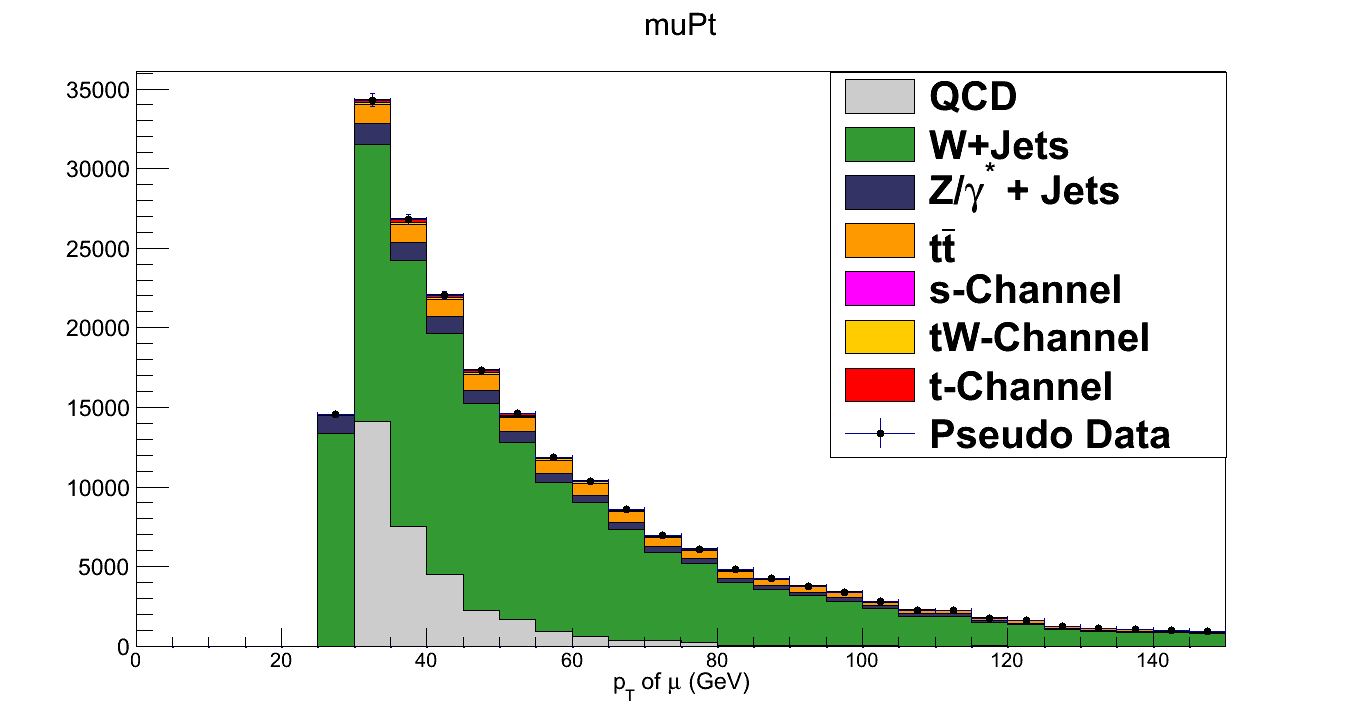
\includegraphics[width=6.5cm]{figures/2J0T/muPt.png}
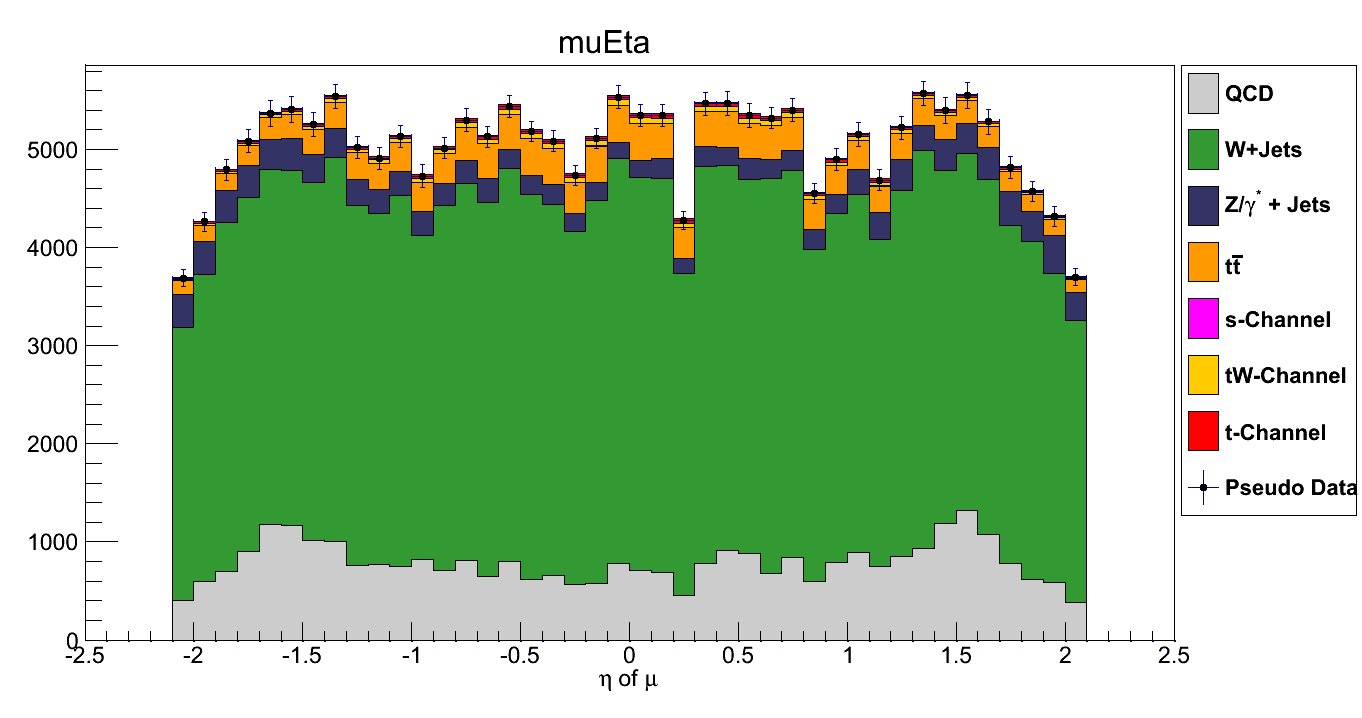
\includegraphics[width=6.5cm]{figures/2J0T/muEta.png}\hfill
\end{center}
\end{figure}
\\
\begin{figure}[hbpt]
\begin{center}
\caption{Leading jet p$_{\rm{T}}$ (left) \& $\eta$ (right) distributions in 2J0T}
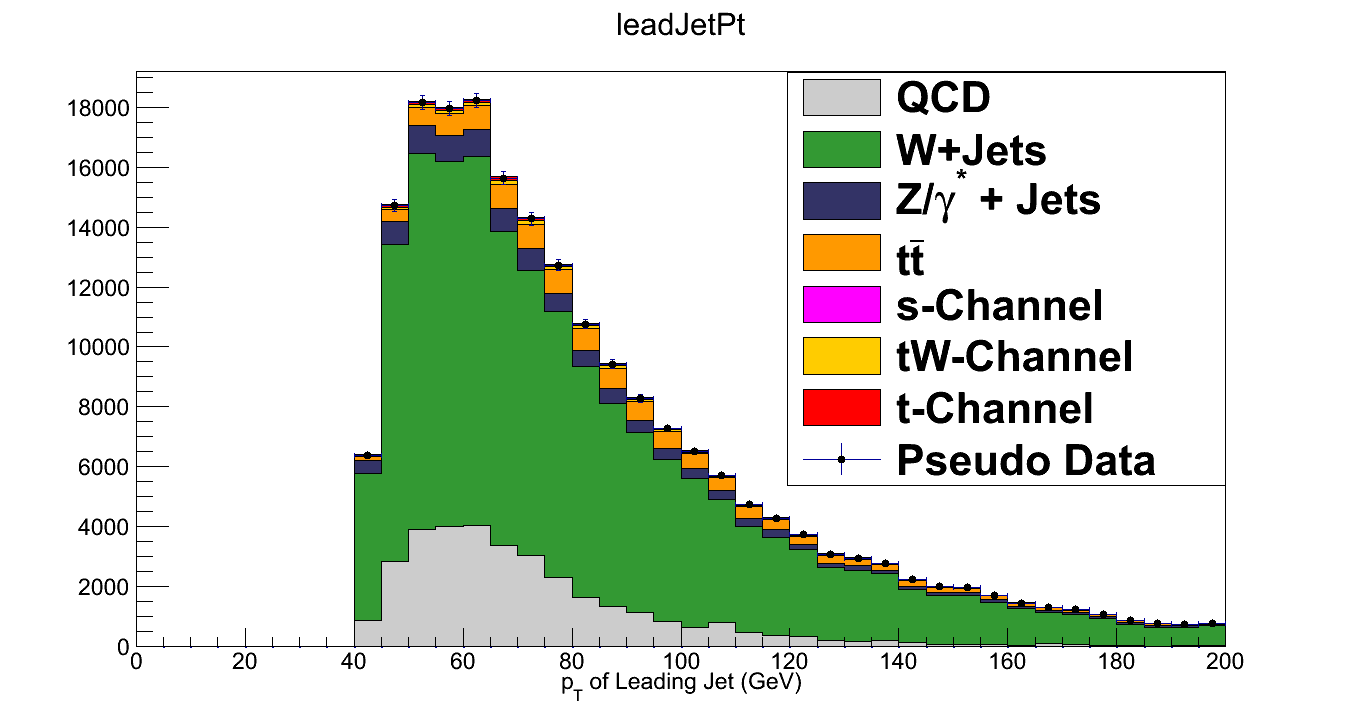
\includegraphics[width=6.5cm]{figures/2J0T/leadJetPt.png}
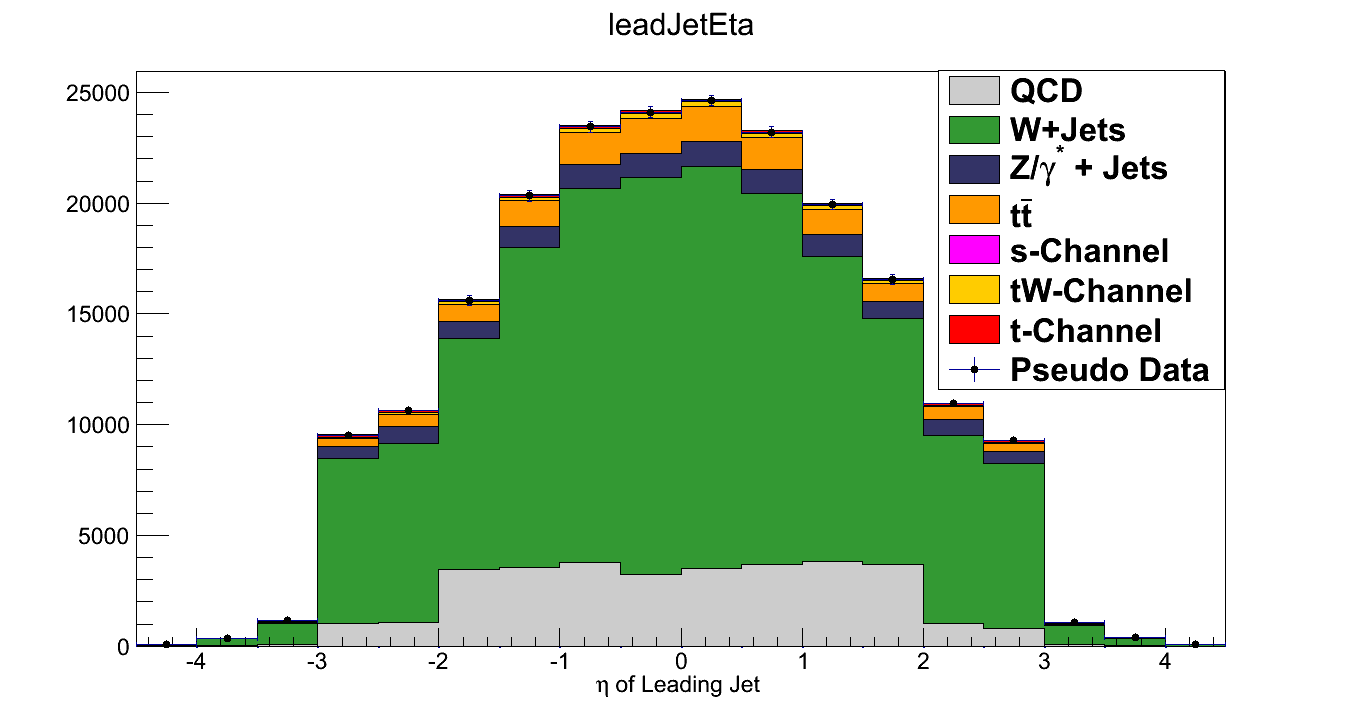
\includegraphics[width=6.5cm]{figures/2J0T/leadJetEta.png}\hfill
\end{center}
\end{figure}
\\
\begin{figure}[hbpt]
\begin{center}
\caption{Sub-leading jet p$_{\rm{T}}$ (left) \& $\eta$ (right) distributions in 2J0T}
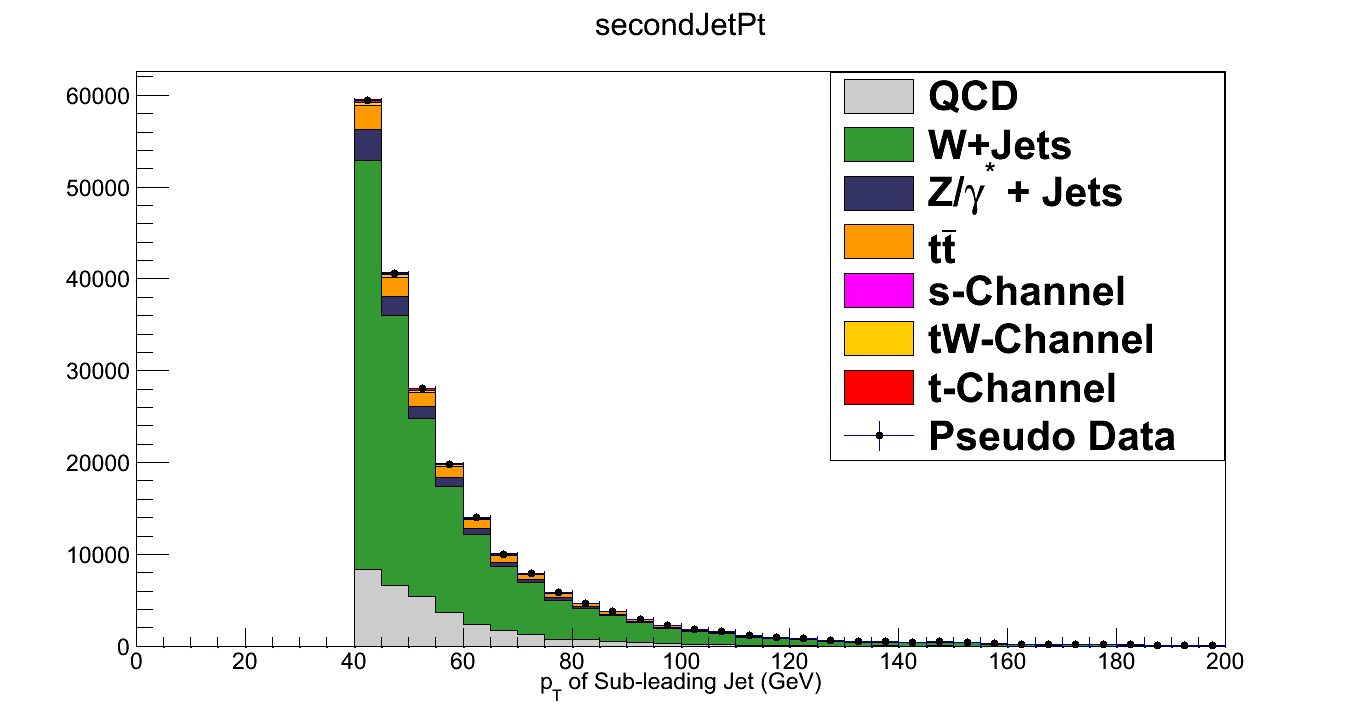
\includegraphics[width=6.5cm]{figures/2J0T/secondJetPt.png}
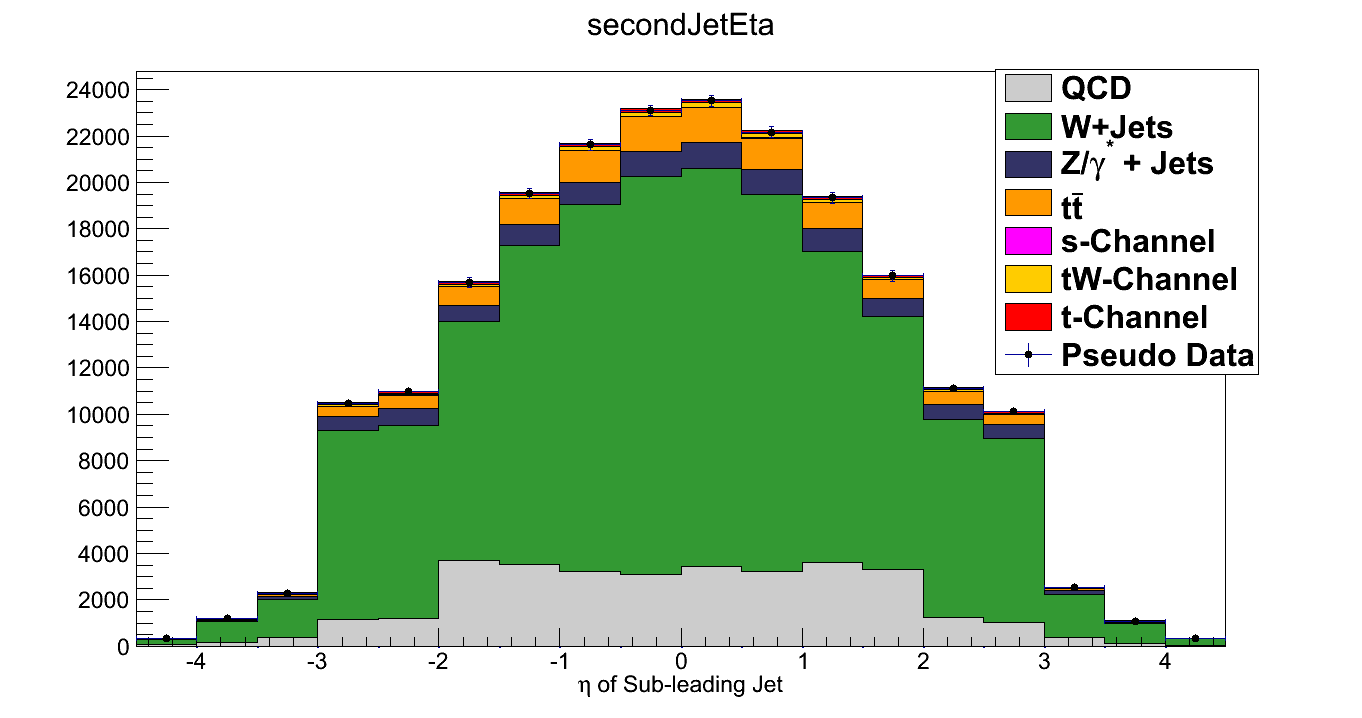
\includegraphics[width=6.5cm]{figures/2J0T/secondJetEta.png}\hfill
\end{center}
\end{figure}

\begin{figure}[hbpt]
\begin{center}
\caption{ Missing E$_{\rm{T}}$ (left) \& m$_{T}$ (right) distributions in 2J0T}
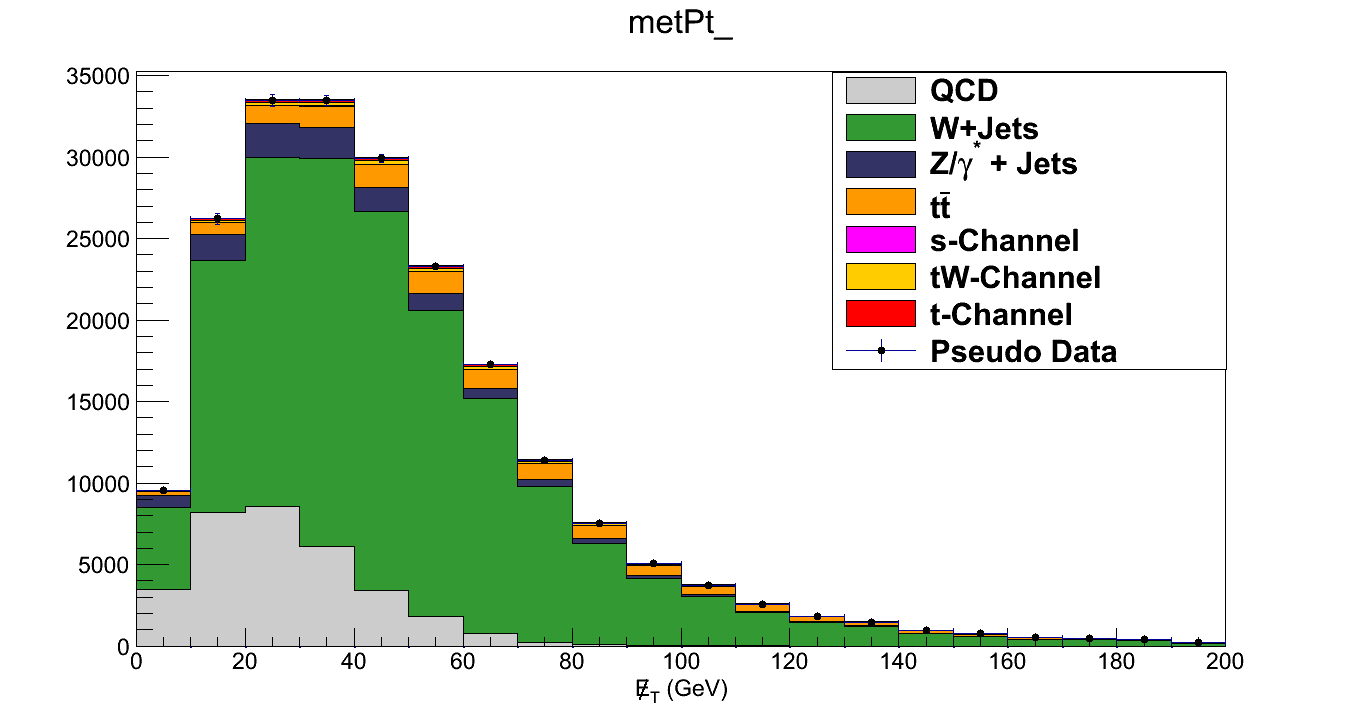
\includegraphics[width=6.5cm]{figures/2J0T/metPt_0To200.png}
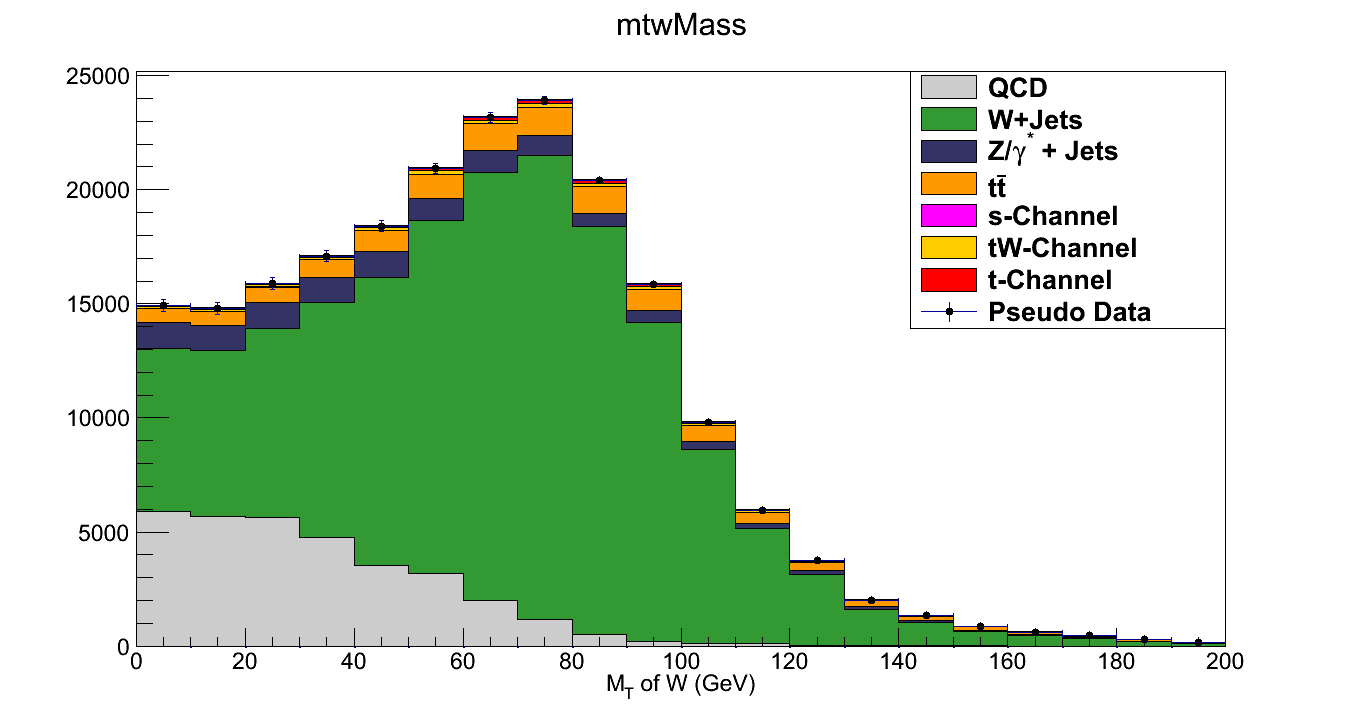
\includegraphics[width=6.5cm]{figures/2J0T/MtW_0To200.png}\hfill 
\end{center}
\end{figure}
\\
\begin{figure}[hbpt]
\begin{center}
\caption{Reconstructed Top Mass distribution in 2J0T}
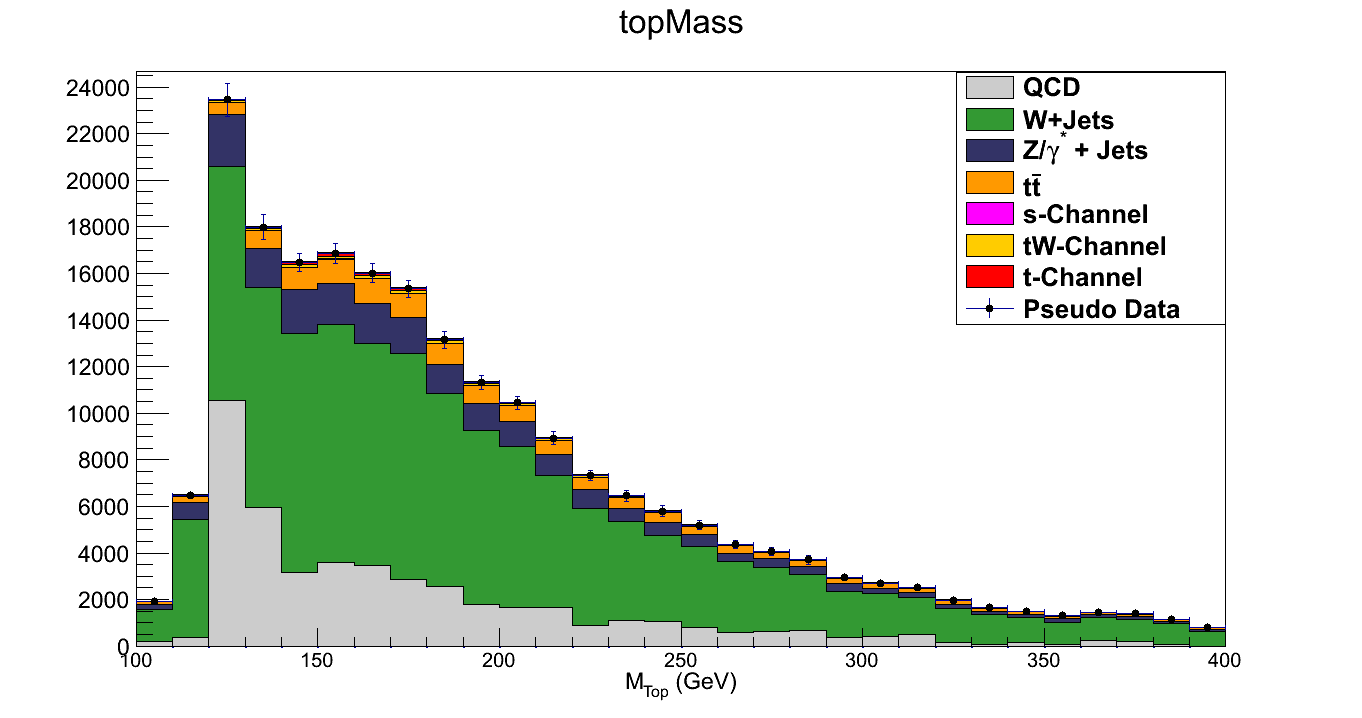
\includegraphics[width=8.0cm]{figures/2J0T/mtop.png}\hfill
\end{center}
\end{figure}
\newpage  
%2Table \ref{tab:2J0T} shows the composition of this sample for muons and electrons. 
%
%\input{yieldTableWSample}
%
%Figure~\ref{fig:2J0TmtwMassMET} shows the W transverse mass distribution (a,b) and the \MET (c,d) for muons (a,c) and electrons (b,d).
%The most disagreement is located where most of the \qcd is located. The treatment of \qcd will be done in Sec~\ref{sec:qcd}, allowing to determine
%from data the \qcd yield.
%
%	\begin{figure}[h]
%	  \begin{center}
%	    \subfigure[]{
%	    \includegraphics[width=0.48\textwidth]{figures/2J_0T_noSyst_noQCDCut_mtwMass_MuStack.png}}
%	    \subfigure[]{
%	    \includegraphics[width=0.48\textwidth]{figures/2J_0T_noSyst_noQCDCut_mtwMass_EleStack.png}}\\
%	    \subfigure[]{
%	    \includegraphics[width=0.48\textwidth]{figures/2J_0T_noSyst_noQCDCut_metPt_MuStack.png}}
%	    \subfigure[]{
%	    \includegraphics[width=0.48\textwidth]{figures/2J_0T_noSyst_noQCDCut_metPt_EleStack.png}}\\
%	    \caption{\label{fig:2J0TmtwMassMET}{Distributions of \mtw (a,c), \met (c,d), in the 2 jets 0 tags sample for muons (a,c) and electrons (b,d).}}
%	  \end{center}
%	\end{figure}
%
%
%In the high \met or \mTW region, representing the qcd depleted region for both variables, we observe a better data-MC agreement in the \met, 
%especially in the electron channel. This motivates us to use the \met for our \qcd determination for electrons.
%
%Figure~\ref{fig:2J0TLepton} shows the lepton \pt and relative isolation after the \qcd rejection cut:
%
%	\begin{figure}[h]
%	  \begin{center}
%	    \subfigure[]{
%	    \includegraphics[width=0.48\textwidth]{figures/2J_0T_noSyst_leptonPt_MuStack.png}}
%	    \subfigure[]{
%	    \includegraphics[width=0.48\textwidth]{figures/2J_0T_noSyst_leptonDeltaCorrectedRelIso_MuStack.png}}\\
%	    \subfigure[]{
%	    \includegraphics[width=0.48\textwidth]{figures/2J_0T_noSyst_leptonPt_EleStack.png}}
%	    \subfigure[]{
%	    \includegraphics[width=0.48\textwidth]{figures/2J_0T_noSyst_leptonRhoCorrectedRelIso_EleStack.png}}\\
%	    \caption{\label{fig:2J0TLepton}{Distributions of \pt (a,b), relative isolation (c,b) in the muon (a,c) and electron (b,d) channel in the 2 jets 0 tags sample after the $\qcd$ cut.}}
%	  \end{center}
%	\end{figure}
%
%Finally, figure ~\ref{fig:2J0TcosthetaLepMET} shows the cosinus of the angle between the lepton and the \MET $cos(\Delta\Phi_{\mu,\MET})$ before (a,b) and after (c,d) the cut for qcd rejection. Such angle is the other component of \mTW besides lepton momentum and missing energy.
%
%	\begin{figure}[h]
%	  \begin{center}
%	    \subfigure[]{
%	    \includegraphics[width=0.48\textwidth]{figures/2J_0T_noSyst_noQCDCut_cosLepMetPhi_MuStack.png}}
%	    \subfigure[]{
%	    \includegraphics[width=0.48\textwidth]{figures/2J_0T_noSyst_noQCDCut_cosLepMetPhi_EleStack.png}}\\
%	    \subfigure[]{
%	    \includegraphics[width=0.48\textwidth]{figures/2J_0T_noSyst_cosLepMetPhi_MuStack.png}}
%	    \subfigure[]{
%	    \includegraphics[width=0.48\textwidth]{figures/2J_0T_noSyst_cosLepMetPhi_EleStack.png}}\\
%	    \caption{\label{fig:2J0TcosthetaLepMET}{Distributions of the cosinus of the angle between the lepton and the \met for muons (a) and electrons(b).}}
%	  \end{center}
%	\end{figure}
%
%Another important variable for the analysis is the reconstructed top mass, for which a jet has to be
%chosen for the top quark decay ansatz. In this sample, the jet with highest value of the track counting
%high purity algorithm is chosen. The reconstructed top mass is shown in figure ~\ref{fig:2J0TtopMass}(a,b).
%
%
%	\begin{figure}[h]
%	  \begin{center}
%	    \subfigure[]{
%	    \includegraphics[width=0.48\textwidth]{figures/2J_0T_noSyst_topMass_MuStack.png}}
%	    \subfigure[]{
%	    \includegraphics[width=0.48\textwidth]{figures/2J_0T_noSyst_topMass_EleStack.png}}
%	    \caption{\label{fig:2J0TtopMass}{Distributions of \mt for muons (a) and electrons(b) in the 2 jets 0 tags sample.}}
%	  \end{center}
%	\end{figure}
%
%
%The pseudorapidity of the jets is a crucial variable for the strategy in this analysis. Fig. \ref{fig:2J0Teta} shows the pseudorapidity distribution 
%of the jet with the lowest value of b-discriminator (henceforth also referred to as ``light jet $\eta$''), while Fig. \ref{fig:2J0Teta_inclusive} 
%shows the pseudorapidity distribution of both jets (henceforth also referred to as ``inclusive jet $\eta$''), in both cases for muons (a) and electrons(b).
%
%	\begin{figure}[h]
%	  \begin{center}
%	    \subfigure[]{
%	    \includegraphics[width=0.48\textwidth]{figures/2J_0T_noSyst_etalj_MuStack.png}}
%	    \subfigure[]{
%	    \includegraphics[width=0.48\textwidth]{figures/2J_0T_noSyst_etalj_EleStack.png}}
%	    \caption{\label{fig:2J0Teta}{Pseudorapidity distributions of the jet with the lowest value of b-discriminator(``light jet $\eta$'') 
%	    in the 2 jets 0 tags sample for muons (a) and electrons (b)}}
%	  \end{center}
%	\end{figure}
%
%	\begin{figure}[h]
%	  \begin{center}
%	    \subfigure[]{
%	    \includegraphics[width=0.48\textwidth]{figures/2J_0T_noSyst_etalj_inclusiveMuStack.png}}
%	    \subfigure[]{
%	    \includegraphics[width=0.48\textwidth]{figures/2J_0T_noSyst_etalj_inclusiveEleStack.png}}
%	    \caption{\label{fig:2J0Teta_inclusive}{Pseudorapidity distributions of both jets in the event(``inclusive $\eta$'') 
%	    in the 2 jets 0 tags sample for muons (a) and electrons (b)}}
%	  \end{center}
%	\end{figure}
%
%Due to the different contributions of the u and d quarks proton $PDF$s,  \wjets processes are not symmetric as function of the lepton charge.
%This feature can be clearly seen in data: Fig. \ref{fig:2J0Tcharge} shows the lepton charge distribution in the sample for muons and electrons.
%There it can also be seen that the asymmetry in data tends to be different with respect to the prediction, thus in the signal extraction procedure the 
%$W$+ jets asymmetry shall be measured simultaneously to $R_{t-channel}$.
%
%Figures ~\ref{fig:2J0Teta_pm} and ~\ref{fig:2J0TtopMass_pm} show the distributions of light jet $\eta$ and \mt divided by charge.
%
%	\begin{figure}[h]
%	  \begin{center}
%	    \subfigure[]{
%	    \includegraphics[width=0.48\textwidth]{figures/charge_2J0T_Mu.pdf}}
%	    \subfigure[]{
%	    \includegraphics[width=0.48\textwidth]{figures/charge_2J0T_Ele.pdf}}
%	    \caption{\label{fig:2J0Tcharge}{Lepton charge in the 2 jets 0 tags sample for muons (a) and electrons (b)}}
%	  \end{center}
%	\end{figure}
%
%	\begin{figure}[h]
%	  \begin{center}
%	    \subfigure[]{
%	    \includegraphics[width=0.48\textwidth]{figures/2J_0T_noSyst_Plus_etalj_MuStack.png}}
%	    \subfigure[]{
%	    \includegraphics[width=0.48\textwidth]{figures/2J_0T_noSyst_Plus_etalj_EleStack.png}}\\
%	    \subfigure[]{
%	    \includegraphics[width=0.48\textwidth]{figures/2J_0T_noSyst_Minus_etalj_MuStack.png}}
%	    \subfigure[]{
%	    \includegraphics[width=0.48\textwidth]{figures/2J_0T_noSyst_Minus_etalj_EleStack.png}}\\
%	    \caption{\label{fig:2J0Teta_pm}{Pseudorapidity distributions of the light jet $\eta$ for positive(a,b) and negative (c,d) charge
%	    leptons in the 2 jets 0 tags sample for muons (a,c) and electrons (b,d)}}
%	  \end{center}
%	\end{figure}
%
%	\begin{figure}[h]
%	  \begin{center}
%	    \subfigure[]{
%	    \includegraphics[width=0.48\textwidth]{figures/2J_0T_noSyst_Plus_topMass_MuStack.png}}
%	    \subfigure[]{
%	    \includegraphics[width=0.48\textwidth]{figures/2J_0T_noSyst_Plus_topMass_EleStack.png}}\\
%	    \subfigure[]{
%	    \includegraphics[width=0.48\textwidth]{figures/2J_0T_noSyst_Minus_topMass_MuStack.png}}
%	    \subfigure[]{
%	    \includegraphics[width=0.48\textwidth]{figures/2J_0T_noSyst_Minus_topMass_EleStack.png}}\\
%	    \caption{\label{fig:2J0TtopMass_pm}{ \mt distributions for positive(a,b) and negative (c,d) charge leptons
%            in the 2 jets 0 tags sample for muons (a,c) and electrons (b,d) }}
%	  \end{center}
%	\end{figure}
